\chapter{Titulo 2}
\label{c2} % la etiqueta para referencias

En los capitulos no usar mas de un nivel de subtitulos....


\subsection{Subcap 1}

\begin{figure}[H]
\begin{center}
   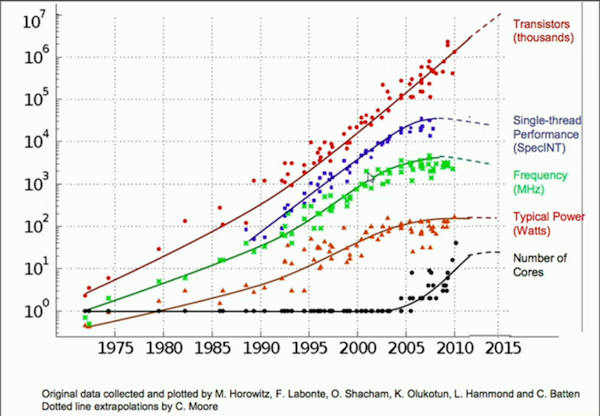
\includegraphics[scale=0.7]{images/c02/moore_and_speed.png}
\end{center}

% texto que aparece al pie de la figura
\caption[Ley de Moore]{La ley de Moore\footnotemark{} se ha cumplido de forma empírica tal como indica la ilustración durante los últimos 40 años. En particular, se evidencia cómo han aumentado la cantidad de transistores en los procesadores. Al mismo tiempo, se observa la tendencia de incrementar el número de núcleos durante los últimos años, sosteniendo la afirmación de que ante la incapacidad de mantener un aumento en la frecuencia del reloj, se ha optado por cambiar las arquitecturas de los procesadores modernos dando paso a esquemas de paralelismo.}
\label{c02_moore_law} % etiqueta para ser usada por referencias desde el texto
\end{figure}
\footnotetext{Fuente: \url{https://www.karlrupp.net/2015/06/40-years-of-microprocessor-trend-data/}}

En los últimos años, se ha experimentado un estancamiento del parámetro de la velocidad del reloj \cite{ross2008cpu}, lo que ha impulsado el desarrollo de arquitecturas más eficientes. Uno de los enfoques por los que se ha inclinado el mercado ha sido el paralelismo. En lugar de tener solo una unidad de cómputo, es que se ha optado por aumentar la cantidad de núcleos distribuyendo así la carga de trabajo en diferentes unidades de cálculo permitiendo de esta manera aumentar el \textit{multi-tasking} y diseñar sistemas energéticamente más eficientes. El paralelismo ha impulsado la necesidad de desarrollar técnicas donde el trabajo realizado por el procesador sea computado por más de un núcleo. Para afrontar el desafío anterior, se debe por un lado, tener una arquitectura de hardware que permita más de un núcleo computacional con la comunicación respectiva entre estos y por otro lado, se debe enfrentar el problema a nivel de software, dividiendo el problema original en tareas más pequeñas para posteriormente reunir las sub-soluciones de cada una de las tareas en la solución general del problema inicial. Es importante mencionar, que no todos los problemas son paralelizables y por lo anterior, no ven un beneficio en dicha arquitectura. Es esperable que en una aplicación computacional se puedan encontrar secciones de código paralelizables y otras que solo pueden implementarse de manera secuencial. Esto resulta que la ganancia máxima que puede otorgar el paralelismo está limitada por lo que se conoce como la Ley de Amdalh \cite{Amdahl:1967:VSP:1465482.1465560}.

\subsubsection{Límites del paralelismo}

Existen dos leyes fundamentales en la computación distribuida las cuales rigen los límites teóricos de ganancia que puede obtener una aplicación al paralelizarse. En primer lugar se encuentra la Ley de Amdalh la cual se define según la fórmula \ref{amdalh_formula}.

\begin{equation}
\label{amdalh_formula}
    S_{latency}\left ( s \right ) = \frac{1}{\left ( 1-p \right ) + \frac{p}{s}}
\end{equation}

Donde:
\begin{itemize}
    \item $S_{latency}$ representa la mejora teórica de la ejecución del programa
    \item $S$ es el beneficio en la sección paralelizable
    \item $P$ es la porción de la ejecución que ve beneficio en el paralelismo
\end{itemize}

Deducible por la misma fórmula es que aún cuando la sección paralelizable vea grandes beneficios, el rendimiento de la ejecución total de la aplicación estará siempre limitada por la sección que no ve beneficio en el paralelismo.
\\
\\
Posteriormente, John L. Gustafson formuló la ley de Gustafson \cite{Gustafson:1988:RAL:42411.42415} donde realizó ciertas revisiones a la ley de Amdalh proponiendo en cambio que la carga de trabajo de la ejecución cambia en la medida que mejoran los recursos disponibles. De esta manera, en la medida que los equipos mejoran, los problemas más grandes se pueden resolver en el mismo tiempo. La formula \ref{gustafson_formula} resume su análisis.

\begin{equation}
\label{gustafson_formula}
    S_{latency}\left ( s \right ) = 1 - p + sp
\end{equation}

Debido al enfoque que toma Gustafson al formular su ley, se puede decir que este es más optimista en cuanto a los beneficios del paralelismo que la ley de Amdalh.





